\section{Datentransformation}
\label{dt}

\subsection{Allgemeine Transformationen}

\begin{itemize}
\item Transformieren des Koordinatensystems $\rightarrow$ Abbildung
\item Seiten des Spielfeldes an $y$-Achse ($x=0$) spiegeln 
\item Zielformat für MATLAB vorbereiten ($x|y|p$)
\end{itemize}

\begin{figure}[H]
\centering
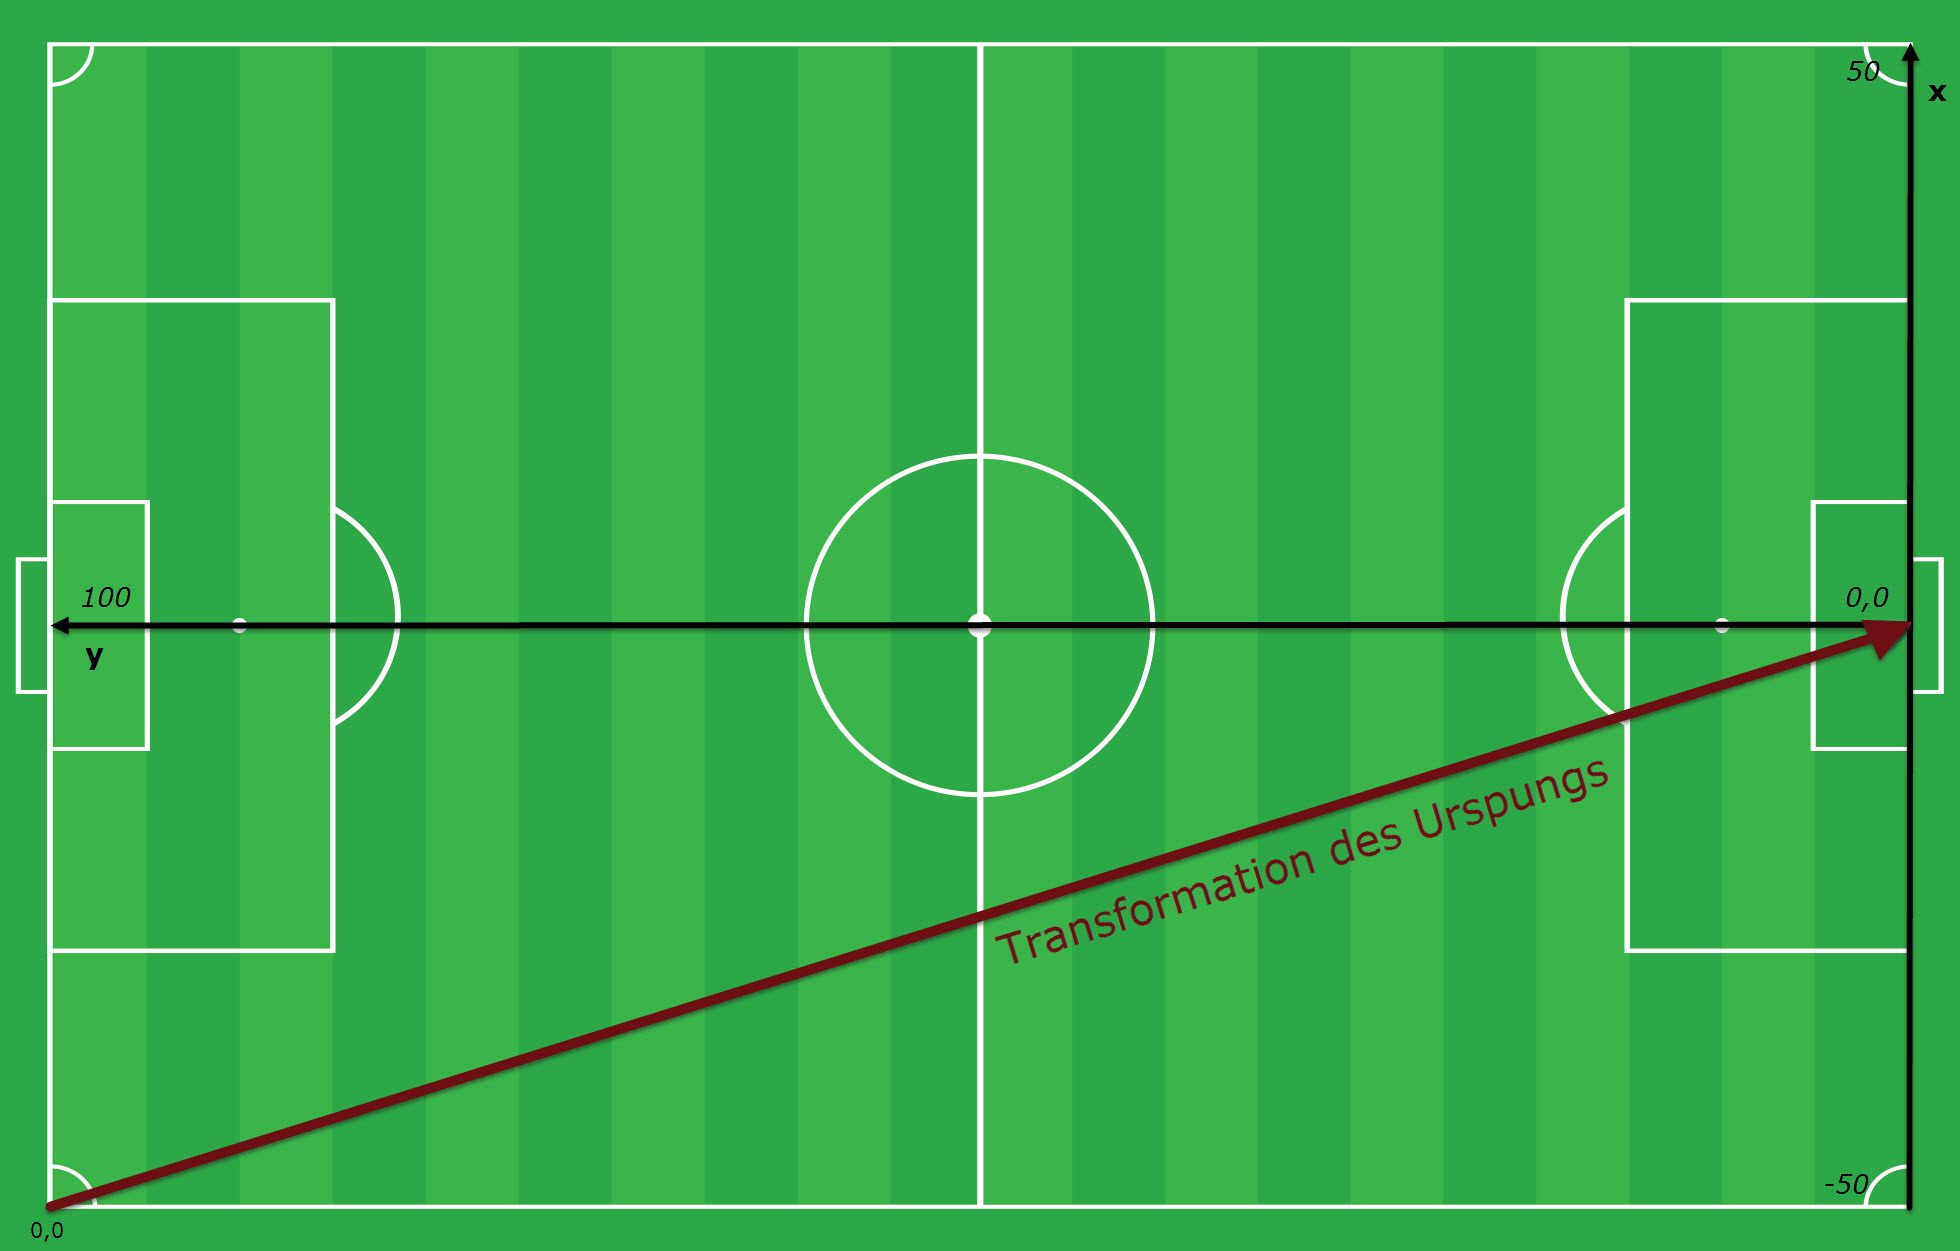
\includegraphics[scale=0.28]{se-wa-jpg/transf_pitch}
\caption[Transformation des Koordinatensystems]{Transformation des Koordinatensystems}
\label{transf_pitch}
\end{figure}


\subsection{Transformation für Winkel- und Distanzbetrachtung}

\begin{itemize}
\item Winkel berechnen
\item Distanz berechnen
\item Einteilung in Intervalle
\item Abbildung der Berechnung
\end{itemize}

\begin{figure}[H]
\centering
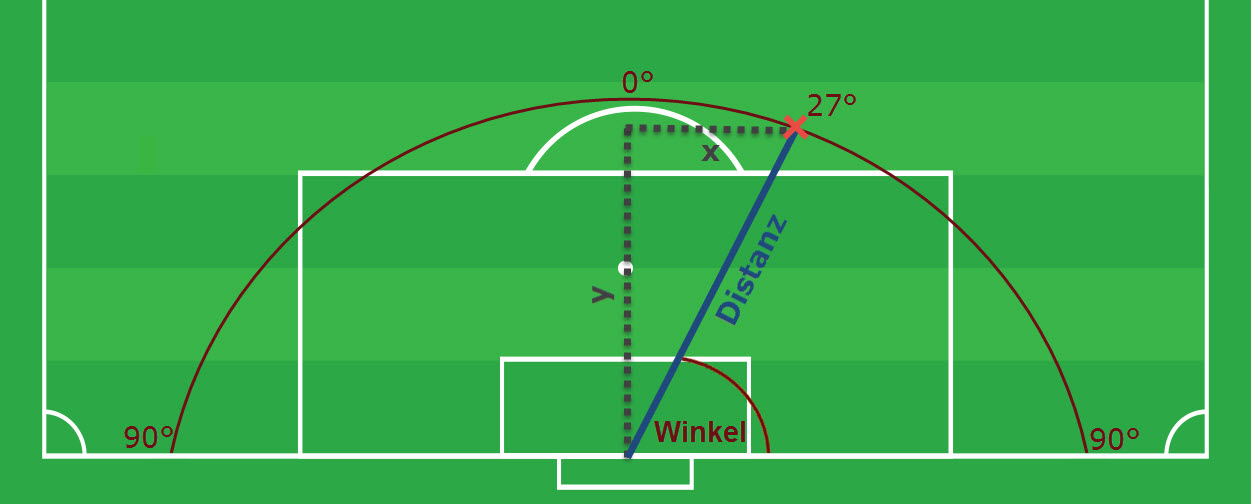
\includegraphics[scale=0.425]{se-wa-jpg/winkel_distanz}
\caption[Berechnung der Distanz und des Winkels]{Berechnung der Distanz und des Winkels}
\label{transf_pitch}
\end{figure}

\begin{equation}
Distanz= \sqrt{x^2 + y^2}
\end{equation}

\begin{equation}
Winkel= \arctan(\frac{|x|}{y})
\end{equation}

\subsection{Transformation für Koordinatenbetrachtung}
\begin{itemize}
\item Spielfeld in Quadrate einteilen $\rightarrow$ Abbildung
\item Wahrscheinlichkeit (p) für jedes Quadrat berechnen $\rightarrow \frac{Anzahl~der~Tore~im~Quadrat}{Gesamtzahl~der~Schüsse~im~Quadrat}$ 
\item Seiten des Spielfeldes an $y$-Achse ($x=0$) spiegeln $\rightarrow$ Durchschnitt der Wahrscheinlichkeiten
\item Zielformat für MATLAB vorbereiten ($x|y|p$)
\end{itemize}

\begin{equation}
p = \frac{Anzahl~der~Tore~im~Quadrat}{Gesamtzahl~der~Schüsse~im~Quadrat}
\end{equation}

\begin{figure}[H]
\centering
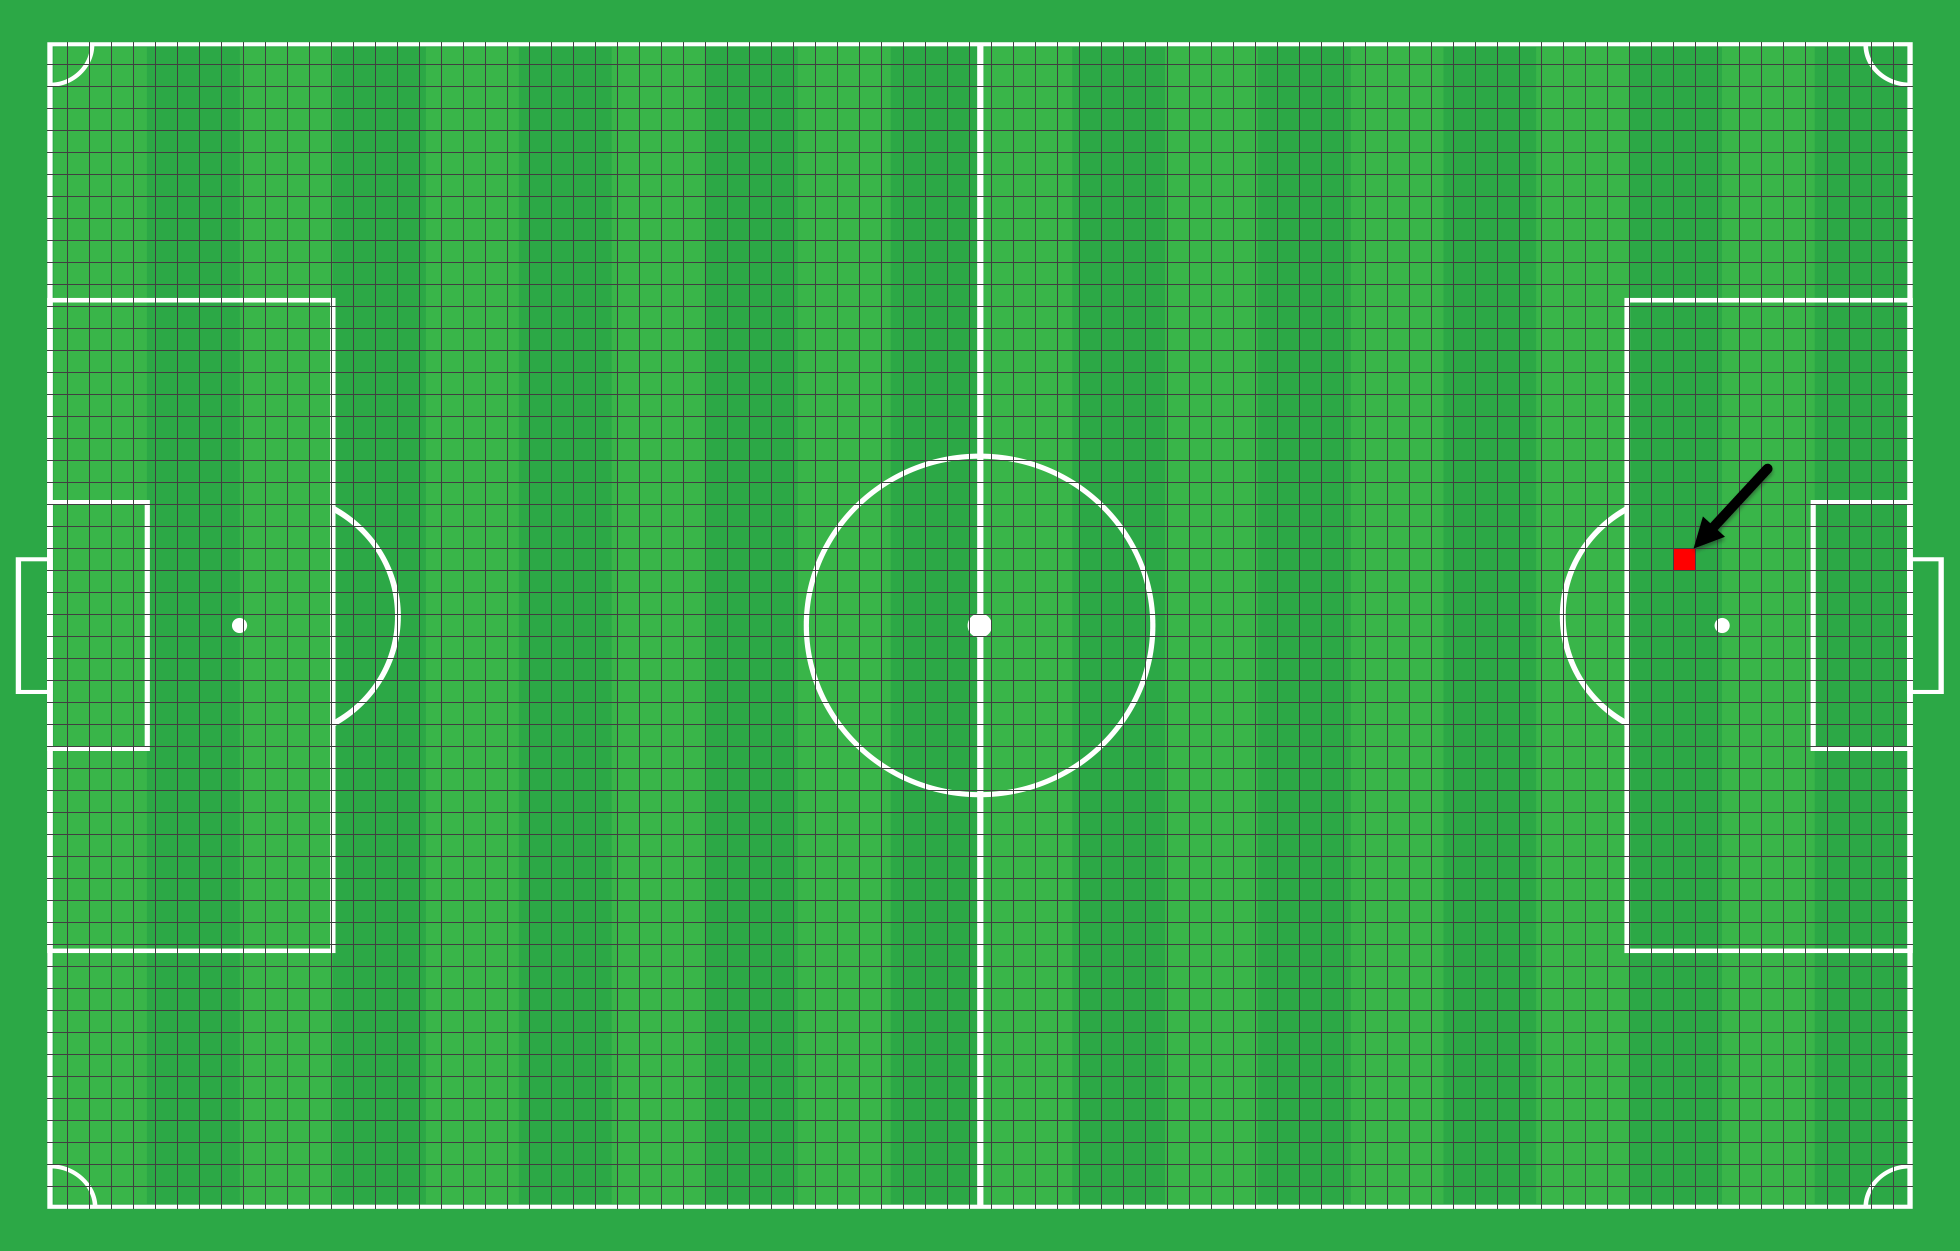
\includegraphics[scale=0.28]{se-wa-jpg/raster}
\caption[Einteilung des Spielfeldes in Raster]{Einteilung des Spielfeldes in Raster}
\label{transf_pitch}
\end{figure}

